\documentclass[xcolor=svgnames]{beamer}
%\usecolortheme[named=Green]{structure}
\usetheme{Boadilla}
\setbeamertemplate{navigation symbols}{}

\def\mycomment#1{{\color{red} #1}}

%%%%%%%%%%%%%%%%%%%%%%%%%%%%%%%%%%%%%%%%%%
%%  Packages
%\def\usetikz#1{}
\def\usetikz#1{#1}
\usepackage{amssymb,amsmath}
\usepackage{graphicx}  %needed for the includegraphics command
%\usepackage{verbatim} % needed for comment environment
%\usepackage{ifthen} % needed for ifthenelse
%\usepackage{hyperref} %for comments
\usepackage{xcolor} %for comments
%\usepackage{enumerate}% for lettering equations
\usetikz{\usepackage{tikz}
\usepgflibrary{arrows}
\usetikzlibrary{calc,through,backgrounds} %****no spaces after commas***
\usetikzlibrary{decorations.pathmorphing}
\usetikzlibrary{decorations.markings}
\usetikzlibrary{positioning} %for below=of xxx syntax in nodes
\usetikzlibrary{backgrounds,fit} %for background layers example
}
%\usepackage[all,arc]{xy} %load this one last
%%%%%%%%%%%%%%%%%%%%%%%%%%%%%%%%%%%%%%%%%%

%%%%%%%%%%%%%%%%%%%%%%%%%%%%%%%%%%%%%%%%%%
%%  Directories
\def\jpgdir{../img}
\def\imgdir{../img}

%%%%%%%%%%%%%%%%%%%%%%%%%%%%%%%%%%%%%%%%%%
%%%%%%%%%%%%%%%%%%%%%%%%%%%%%%%%%%%%%%%%%%
%% Version 5
%    Jan 3, 2013
%       Added \subhead, \problem, \numexamp
%    Feb 27, 2012
%       Added \xbar, \Var, \Cov  macros
%    Feb 11, 2012
%       Reorganized to use with header.tex and new mkpdf.sh
%       added some macros
%    Feb 5, 2012
%       Copied from 18.03
%       Added myhide code.
%       Removed topics codes
%%%%%%%%%%%%%%%%%%%%%%%%%%%%%%%%%%%%%%%%%%

%%  Macros
\def\partHeading#1#2{\mcent{\textrm{\large \bf Part #1 \hspace{2.3ex}#2}}}


%%  Simple macros
\def\mycomment#1{{\color{red}#1}}
\def\mcent#1{\hspace*{\stretch{1}}#1\hspace*{\stretch{1}}{ }}
\def\hs#1{\hspace*{#1 ex}}
\def\nl#1{\\[.#1ex]}
\def\ds{\displaystyle}
\def\cont{\vspace*{\stretch{1}}\emph{(continued)} \newpage}
\def\reading{\textbf{Reading. }}
\def\examples{\textbf{Examples. }}
\def\example{\textbf{Example. }}
\def\examp#1{\textbf{Example #1. }}
\def\problem{\textbf{Problem. }}
\def\problems{\textbf{Problems. }}
\def\subhead#1{\textbf{#1.}}
\def\indetop#1#2#3{\stackrel{\; \scriptstyle{{#1}{#3}{#2}}}{=} \;}
\def\indet#1#2{\stackrel{\scriptstyle{\; \frac{#1}{#2}}}{=} \;}
\def\indetzero{\indet{0}{0}}
\def\indetinf{\indetop{\infty}{\infty}{/}}
\def\qedbox{\rule{1ex}{1ex}}

\def\mybull{$\bullet$}
\def\W{\Omega}
\def\w{\omega}
\def\mycap{\,\cap\,}
\def\mycup{\,\cup\,}
\def\Norm{\text{N}}

\def\myref#1{(\ref*{#1})}

\def\mypart#1#2{\frac{\partial #1}{\partial #2}}
%      fully specified partial
\def\fp#1#2#3{(\partial #1/\partial #2)_{#3}}                %without \frac
\def\ffp#1#2#3{\left.\frac{\partial #1}{\partial #2}\right|_{#3}}  %with \frac
\def\mpp#1#2#3{\left(\mypart{#1}{#2}\right)_{#3}} 
\def\myderiv#1#2{\frac{d#1}{d#2}}
\def\mynderiv#1#2#3{\frac{d^{#3}#1}{d#2^{#3}}}
\def\mygrad{\boldsymbol{\nabla}}         %gradient
\def\gf#1#2{\left.\mygrad #1\right|_{#2}}
\def\endandindent{\\ \hspace*{20pt}}
\def\e#1{\mathrm{e}^{#1}}
\def\myIm{\textup{Im}}
\def\myRe{\textup{Re}}
\def\conj#1{\overline{#1}}
\def\tran{^\mathrm{T}}
\def\ans{{\bf \underline{answer:}}{ }}
\def\th{$^{\mathrm{th}}$}
\def\myhead#1{\noindent \textbf{#1}}
\def\tbf#1{\textbf{#1}}
\def\mysep{: }
\def\lap{{\mathcal{L}}}
\def\ilap{\lap^{-1}}
\def\myimply{\; \Rightarrow \;}
\def\myequiv{\; \Leftrightarrow \;}
\def\ft{\hat}
\def\xbar{\overline{X}}
\def\Var{\textup{Var}}
\def\Cov{\textup{Cov}}
\def\bypartshelp#1#2#3#4#5#6#7{\framebox{$\begin{array}[#7]{lll} 
#5=#1 & d#6=#2\\
d#5=#3 & #6=#4 \end{array}$}}
\def\byparts#1#2#3#4{\bypartshelp{#1}{#2}{#3}{#4}{u}{v}{l}}
\def\bypartst#1#2#3#4{\bypartshelp{#1}{#2}{#3}{#4}{u}{v}{t}}

%matlab 
\newcommand{\mlcmd}[2]{\textgreater{} \texttt{#1}\\ \texttt{#2}\\}
\newcommand{\mlcmdna}[1]{\textgreater{} \texttt{#1}\\}
\newcommand{\mlans}[2]{#1 =\\[.5ex]\hs3\parbox{5in}{#2}}
\def\mlcomm#1{{\color{blue}\% #1}\\}
\def\mlinstr#1{\mlcomm{#1}}
\def\mlcar{\^{ }}

%counters
\newcounter{examplectr}
\setcounter{examplectr}{1}
\renewcommand{\theexamplectr}{\arabic{examplectr}}
\newcommand{\numexamp}{\textbf{Example \arabic{examplectr}.{ }}\addtocounter{examplectr}{1}}

%matrices
\def\defleftbrace{(}
\def\defrightbrace{)}
\def\twobytwohelp#1#2#3#4#5#6#7{\left#6 \begin{array}{#1} #2 & #3 \\ #4 & #5 \end{array} \right#7}
\def\twobytwo#1#2#3#4{\twobytwohelp{rr}{#1}{#2}{#3}{#4}{\defleftbrace}{\defrightbrace}}
\def\twobytwoc#1#2#3#4{\twobytwohelp{cc}{#1}{#2}{#3}{#4}{\defleftbrace}{\defrightbrace}}
\def\twobytwodet#1#2#3#4{\twobytwohelp{rr}{#1}{#2}{#3}{#4}{|}{|}}
\def\twobytwodetc#1#2#3#4{\twobytwohelp{cc}{#1}{#2}{#3}{#4}{|}{|}}
\def\twobyonehelp#1#2#3{\left\defleftbrace \begin{array}{#1} #2\\ #3  \end{array} \right\defrightbrace}
\def\twobyone#1#2{\twobyonehelp{r}{#1}{#2}}
\def\twobyonec#1#2{\twobyonehelp{c}{#1}{#2}}
\def\threebythree#1#2#3#4#5#6#7#8#9{\left\defleftbrace \begin{array}{rrr} #1&#2&#3\\ #4&#5&#6\\ #7&#8&#9 \end{array} \right\defrightbrace}
\def\threebythreec#1#2#3#4#5#6#7#8#9{\left\defleftbrace \begin{array}{ccc} #1&#2&#3\\ #4&#5&#6\\ #7&#8&#9 \end{array} \right\defrightbrace}
\def\threebythreedet#1#2#3#4#5#6#7#8#9{\left| \begin{array}{rrr} #1&#2&#3\\ #4&#5&#6\\ #7&#8&#9 \end{array} \right|}
\def\threebythreedetc#1#2#3#4#5#6#7#8#9{\left| \begin{array}{ccc} #1&#2&#3\\ #4&#5&#6\\ #7&#8&#9 \end{array} \right|}
\def\threebyone#1#2#3{\left\defleftbrace \begin{array}{r} #1\\ #2\\ #3 \end{array} \right\defrightbrace}
\def\threebyonec#1#2#3{\left\defleftbrace \begin{array}{c} #1\\ #2\\ #3 \end{array} \right\defrightbrace}
\def\threebytwo#1#2#3#4#5#6{\left\defleftbrace \begin{array}{rr} #1&#2\\ #3&#4\\ #5&#6 \end{array} \right\defrightbrace}
\def\threebytwoc#1#2#3#4#5#6{\left\defleftbrace \begin{array}{cc} #1&#2\\ #3&#4\\ #5&#6 \end{array} \right\defrightbrace}

%Vectors and line segments
\def\vb#1{\mathbf{#1}}  %bold
\def\va#1{\overrightarrow{#1}}  %arraow
\def\vba#1{\overrightarrow{\mathbf{#1}}}  %bold/arraow
\def\vl#1{\overline{#1}} %overline
\def\vbl#1{\overline{\mathbf{#1}}} %bold/overline
\def\vu#1{\widehat{#1}} %unit vector
\def\vbu#1{\widehat{\mathbf{#1}}} %bold/unit vector
\def\un#1{\frac{#1}{\left|#1\right|}}  %normalize vector
\def\vbi{\vbu{i}}
\def\vbj{\vbu{j}}
\def\vbk{\vbu{k}}
\def\vc#1{\langle #1 \rangle}
\def\vcb#1{\left\langle #1 \right\rangle}

\newcommand{\st}[1]{\ensuremath{^{\scriptstyle \textrm{#1}}}}
\newcommand{\undertext}[1]{\ensuremath{\underline{\textrm{#1}}}}
\newcommand{\fracc}{\displaystyle\frac}
\newcommand{\summ}{\displaystyle\sum}

%%%%%%%%%%%%%%%%%%%%%%%%%%%%
%% tikz
\usetikz{\tikzset{
addarrow/.style={postaction={decorate},
        decoration={markings,mark=at position #1 with {\arrow{>}}}}
}}

%%%%%%%%%%%%%%%%%%%%%%%%%%%
%% Sample Complex formatting macros
%\makeatletter
%\renewcommand\section{\goodbreak\@startsection {section}{1}{\z@}%
%%%                                   {-3.5ex \@plus -1ex \@minus -.2ex}%
%                                   {-3.5ex \@plus -1ex \@minus -.2ex}%
%                                   {2.3ex \@plus.2ex}%
%                                   {\normalfont\large\bfseries%
%                                     \centering\sectionname\ }}

%\renewcommand\subsection{\goodbreak\@startsection{subsection}{2}{\z@}%
%%                                     {-3.25ex\@plus -1ex \@minus -.2ex}%
 %                                    {-2ex\@plus -1ex \@minus -.2ex}%
%%                                     {1.5ex \@plus .2ex}%
%                                     {1.25ex \@plus .2ex}%
%                                     {\normalfont\large\bfseries}}
%\makeatother

%\renewcommand{\thesection}{\Roman{section}}
%\newcommand\sectionname{Part}
%\newcommand{\alphalist}{% changes enumerate 1st level to (a)...(z)
%  \renewcommand{\theenumi}{\alph{enumi}}%
%  \renewcommand{\labelenumi}{\theenumi)}%
%}
%\alphalist
%%%%%%%%%%%%%%%%%%%%%%%%%%%%%%%%%%%%%%%%%%

\usepackage{ifthen} % needed for ifthenelse

\def\needstobedone{XXX***XXX}

\def\whichterm{Spring 2013}
%\def\whichprogram{ESG}
\def\teacher{Dr. Jeremy Orloff and Dr. Jonathan Bloom}
\def\email{jorloff}

%\def\website{web.mit.edu/jorloff/www/18.05}
%\def\matlabadd{\intentionalerror{need matlab dir}}
%\def\matlabdir{\intentionalerror{need matlab dir}}

\def\wheredue{in 2-285{}}
%\def\finalinfo{To be anounced}

\def\psdue#1{\textbf{Pset #1 due}}
%\def\exam#1#2{\textbf{Exam #1: covering #2}}
%\def\review{Discussion, review and catch up.}
%\def\reviewentry#1#2{\textbf{Continuation: } (#1) \, #2}
%\def\recitationentry#1#2{\textbf{Problem section:} (#1) \, #2}

%\def\examonecovers{\intentionalerror}
%\def\examtwocovers{\intentionalerror}

%Problem set due dates
\def\duetime{4:30 PM}
\def\psonedue{Monday, Feb. 11 at \duetime}
\def\pstwodue{Tuesday, Feb. 19 at \duetime}
\def\psthreedue{Monday, Feb. 25 at \duetime}
\def\psfourdue{Monday, Mar. 4 at \duetime}
\def\psfivedue{Monday, Mar. 18 at \duetime}
\def\pssixdue{Monday, Apr. 8 at \duetime}
\def\pssevendue{Wednesday, Apr. 17 at \duetime}
\def\pseightdue{Monday, Apr. 29 at \duetime}
\def\psninedue{Monday, May 6 at \duetime}
\def\pstendue{Not to be turned in}

\def\psetblurb{You are encouraged to discuss the problem sets with each other.
You must either list any collaborators or write "no collaborators" at the 
top of your paper.
You may \emph{not} read another student's paper for help with a problem.
You must write your solutions in your own words.}




%%%%%%%%%%%%%%%%%%%%%%%%%%%%%%%%%%%%%%%%%%



\def\myat{\makeatletter@\makeatother}
\def\myheart{{\color{red} \heartsuit}}
\def\mydiamond{{\color{red} \diamondsuit}}

%%%%%%%%%%%%%%%%%%%%%%%%%%%
\date{February 5, 2013}
\author{18.05 Class 1}

%%%%%%%%%%%%%%%%%%%%%%%%%%%

%%% Reminder
% you can define \title, \subtitle, \institute etc in the preamble
% and then get a title \begin{frame}\titlepage \end{frame}


\begin{document}

%--- the titlepage frame -------------------------%
\begin{frame}[plain]
\begin{center} 
\Large \color{blue} Welcome to 18.05\\
Introduction to Probability and Statistics\\
Spring 2013
\end{center}

\mcent{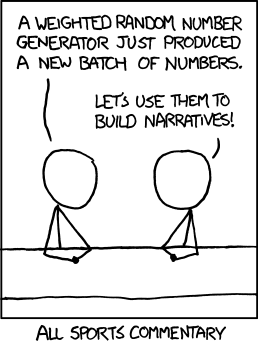
\includegraphics[height=2.5in]{\imgdir/sportsxkcd.png}}

\end{frame}

\begin{frame}{Staff}
\begin{itemize}

\item {\Large Jeremy (Jerry) Orloff}\\jorloff\myat mit.edu, office hours M 1-3 in 24-606\\
\item {\Large Jonathan (Jon) Bloom}\\jbloom\myat math.mit.edu, office hours \emph{TBA}\\
\item {\Large Sameer Deshpande}\\sameerd\myat mit.edu, office hours \emph{TBA}\\
\item {\Large Shelby Heinecke}\\shelbyh\myat mit.edu, office hours \emph{TBA}
\end{itemize}
\end{frame}

\begin{frame}{MITx/18.05x}

{\large You should have received this information in an email.\\
If you did not see us after class.}

\bigskip

\begin{itemize}
\item We'll use the MITx platform:  {\bf \color{blue} https://lms.mitx.mit.edu}
\item The 18.05 Stellar site has a link to MITx
\item Sign up using your MIT email address.
\item \textbf{Do not} log in, just click find courses; then choose 18.05x.
\end{itemize}

Our Stellar site has a link to MITx\\

\begin{itemize}
\item Site will have all reading materials and problem sets
\item Solutions to all problems discussed in class will be posted\\ 
here after class
\end{itemize}
\end{frame}

\begin{frame}{Active Learning}

{\large
Read the 'Information Policy and Goals' on our MITx site.

\bigskip

Before class
\begin{itemize}
\item Reading and reading questions.
\item Reading questions count toward grade.
\item Lecture will assume you've done the reading.
\end{itemize}

In class:
\begin{itemize}
\item Combination of lecture and problem solving
\item We won't assume you've completely mastered the reading. 
  \begin{itemize}
  \item Will assume a level of familiarity. 
  \item Use the discussion boards on the MITx/18.05x site.
  \item Bring questions to class.
    \end{itemize}
\end{itemize}
}
\end{frame}

\begin{frame}{Class}
Read the 'Information Policy and Goals' on our MITx/18.05x site.\\[2ex]

\textbf{Class Time}
\begin{itemize}
\item TR: Lecture/clicker questions/table questions\\
Participation on clicker questions counts towards your grade
\item F: Studio -- bring your laptop
\end{itemize}

\bigskip

\textbf{In-class Groups}
\begin{itemize}
\item At the end of week 2 we will form permanent groups of 3 and make seating assignments.
\item You will be able to choose your own group.
\item If you need to find a group or your group needs a third person let us know and we'll help.
\end{itemize}

\bigskip
\textbf{Matlab}: for computation, simulation and visualization
\begin{itemize}
\item will teach you everything you need 
\item no hardcore programming.
\end{itemize}
\end{frame}


\begin{frame}{Problem Sets}

{\Large
\begin{itemize}
\item Usually due on Mondays
\item Turn in to 2-285 by 4:30 PM\\ 
\item You'll be able to check your numerical answers to \\
problems on the MITx/18.05x site before the due date.
\item Problem sets will be graded on your explanation of 
your answer.
\end{itemize}
}
\end{frame}

\begin{frame}{Clickers and Matlab}

{\LARGE Clickers}

{\Large
Buy a TurningTechnology clicker at MIT coop.

Follow the instructions for registering it to this class in
the Information, Policies and Goals section of MITx/18.05x\\

\bigskip
\bigskip
     
{\LARGE Matlab}

Free for MIT students. 

Instructions and a link for this are on MITx/18.05x.
}

\end{frame}

\begin{frame}{Information, Policies and Goals}

{\Large Everything we just went over and more is in the 

\bigskip

Information, Policies and Goals section of MITx/18.05x
}
\end{frame}

\begin{frame}{For Next Time}

{\Large
\begin{itemize}
\item Familiarize yourself with the MITx/18.05x site
\item Get and register clicker
\item Install Matlab\\\phantom{xxx}
\item Read class 1 notes (summary of what we'll do today)
\item Go through the class 2 sequence and answer the\\ 
  reading questions
\end{itemize}
}
\end{frame}

\begin{frame}{Probability vs. Statistics}

{\Large
Different subjects: both about random processes

\bigskip

Probability
\begin{itemize}
\item Logically self-contained
\item A few rules for computing probabilities
\item One correct answer
\end{itemize}

Statistics
\begin{itemize}
\item Messier and more of an art
\item Get experimental data and try to draw probabilistic conclusions
\item No single correct answer
\end{itemize}
}
\end{frame}

\begin{frame}{Counting: Motivating Examples}

{\Large
What is the probability of getting exactly 1 heads in 3 tosses of
a fair coin?

}

\end{frame}

\begin{frame}{Poker Hands}
Deck of 52 cards
\begin{itemize}
\item 13 \emph{ranks}: 2, 3, $\dots$, 9, 10, J, Q, K, A
\item  4 \emph{suits}: $\myheart,  \spadesuit, \mydiamond, \clubsuit,$
\end{itemize}

Poker hands
\begin{itemize}
\item Consists of 5 cards
\item A {\em one-pair} hand consists of two cards having one rank and the remaining three cards having three other rank
\item Example: $\{2 \myheart, 2 \spadesuit, 5 \myheart, 8 \clubsuit, \text{K} \mydiamond\}$ 

\end{itemize}


The probability of a one-pair hand is: \\
1) less than 5\%\\
2) between 5\% and 10\% \\
3) between 10\% and 20\%\\
4) between 20\% and 40\% \\
5) greater than 40\% \\
\end{frame}

\begin{frame}{Sets in Words}
$S$ = \{Jan, Feb, Mar, Apr, May, Jun, Jul, Aug, Sep, Oct, Nov, Dec\}\nl5
\bigskip

$L$ = the month has 31 days = \{Jan, Mar, May, Jul, Aug, Oct, Dec\}\nl5
\bigskip

$R$ = the month's name 'r' = \{Jan, Feb, Mar, Apr, Sep, Oct, Nov, Dec\}
\bigskip

$L\mycap R$ = \{Jan, Mar, Oct, Dec\} = months with 31 days and an `r'
\end{frame}

\begin{frame}{Visualize Set Operations with Venn Diagrams}


\includegraphics{\imgdir/figc1-1.pdf}
\end{frame}

\begin{frame}{DeMorgan's Laws}

{\LARGE
\mcent{$(L \mycap R)^c = L^c \mycup R^c$}

\bigskip

\mcent{$(L \mycup R)^c = L^c \mycap R^c$}
}
\end{frame}

\begin{frame}{Product of Sets}

{\LARGE
\mcent{ $S\times T = \{(s,t)\}$}
}

\end{frame}

\begin{frame}{Inclusion-Exclusion Principle}
\mcent{\includegraphics{\imgdir/figc1-3.pdf}}
\end{frame}

\begin{frame}{Table Question}

{\Large
A band consists of singers and guitar players.

\begin{itemize}
\item 7 people sing
\item 4 play guitar
\item 2 do both
\end{itemize}

How many people are in the band?
}
\end{frame}

\begin{frame}{Rule of Product}

{\Large

\bigskip
\bigskip

\mcent{3 shirts, 4 pants = 12 outfits}

\bigskip
\bigskip
\bigskip
\bigskip

\bigskip
(More powerful than it seems.)
}
\end{frame}

\begin{frame}{Table Question}

{\Large
There are 5 Competitors in 100m final. 

\medskip

How many ways can gold silver and bronze be awarded?
}

\bigskip
\mcent{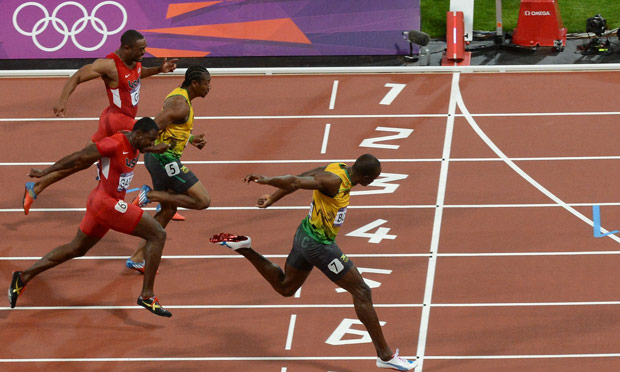
\includegraphics[width=3in]{\imgdir/Usain-Bolt-wins-011.jpg}}

\end{frame}

\begin{frame}{Permutations}

{\Large Lining things up. How many ways can you do it? 

\bigskip
\bigskip

`abc' \,  and \, `cab' \, are different permutations of \{a, b, c\}

}


\end{frame}

\begin{frame}{Permutations of $k$ from a set of $n$}

{\Large
Give all permutations of 3 things out of $\{a,b,c,d\}$

}

\end{frame}

\begin{frame}{Permutations of $k$ from a set of $n$}

{\Large
Give all permutations of 3 things out of $\{a,b,c,d\}$
\bigskip

\[ \begin{array}{llllllllllllllll}
abc & abd & acb & acd & adb & adc \\
bac & bad & bca & bcd & bda & bdc \\
cab & cad & cba & cbd & cda & cdb \\
dab & dac & dba & dbc & dca & dcb
\end{array}
\]

\bigskip
 Would you want to do this for 7 from a set of 10?

}
\end{frame}

\begin{frame}{Combinations}

{\Large
Choosing subsets -- order doesn't matter. 

\bigskip

How many ways can you do it?
}
\end{frame}

\begin{frame}{Combinations of $k$ from a set of $n$}

{\Large
Give all combinations of 3 things out of $\{a,b,c,d\}$

\bigskip
\bigskip
\bigskip

\textbf{Answer:} \, \{a,b,c\}, \{a,b,d\}, \{a,c,d\}, \{b,c,d\}
}

\end{frame}

\begin{frame}{Permutations and Combinations}

{\Large
\[ \begin{array}{llllllllllllllll}
abc & acb & bac & bca & cab & cba & \quad & \{a,b,c\}\\
abd & adb & bad & bda & dab & dba & \quad & \{a,b,d\}\\
acd & adc & cad & cda & dac & dca & \quad & \{a,c,d\}\\
bcd & bdc & cbd & cdb & dbc & dcb & \quad & \{b,c,d\}\\[.8ex]
\multicolumn{6}{c}{\text{Permutations: }_4P_3} && 
\text{Combinations: }_4C_3
\end{array}
\]

\bigskip

\[_4C_3 = \frac{_4P_3}{3!}\]

}
\end{frame}

\begin{frame}{Table Question}

{\Large
a) Count the number of ways to get exactly 3 heads in 10 flips of a coin.

\bigskip

b) For a fair coin, what is the probability of exactly 3 heads in 10 flips?

}

\end{frame}
\end{document}

